\subsection{Ray tracing simulations}

\textbf{You will:}

\begin{itemize}
    \item Use different mirror shapes in SHADOW
    \item Experience with the automatic calculation of the mirror parameters
    \item Include mirror reflectivity
\end{itemize}

\textbf{Questions:}

Create a geometrical source with Gaussian shape (sx=57 um, sz=10.4 um) and Gaussian divergence (sx’=88.5 urad and sz’=7.2 urad) to simulate the emission of an ESRF 1.65 m undulator at 10 keV in a Low beta section.

\textbf{i)} Study the case of different mirror shapes (spherical, toroidal and ellipsoidal) for focusing the source with distances (p,q)=(30m,10m) (magnification 1/3) and (30m,1m) (magnification 1/30). Set the grazing angle to 2 mrad. Study the effect of the spherical aberrations and its influence depending on the magnification factor. 
Study the dependence on mirror dimensions and incident angle. 

\textbf{ii)} Enter the effect of mirror reflectivity for the Ellipsoidal mirror at M=1/3. Consider a Rh (density=12.4 g/cm3) coating and a source with energy distribution in 5-45 keV (box-distribution). 
Define mirror finite dimensions 0.2 $\times$ 1 m$^2$ (center it well, footprint is nor symmetric).
Plot also the intensity versus energy.

\textbf{Hints:} 
The workspace file {\tt aberrations.ows} contains the workflow of this exercise. 




\textbf{Notes:}
For the different mirrors, shadow4 can calculate the surface parameters (curvature radii, ellipse axes, etc). by selecting the parameters in Basic Settings → Surface Shape -> Type =  “internal/calculated” . The resulting mirror parameters can be seen using the ``Info" widget (“OE Info” tab). For including reflectivity, you can define internally using either the ``xraylib" or ``DABAX" library. Alternatively, you can use the preprocessor ``PreRefl" for creating the material file. 


\textbf{Answer}

i) 

The aberrations effect increases if
\begin{itemize}
\item one goes to more grazing angle
\item one reduces the magnification factor (i.e., mode demagnification of the source)
\item one uses larger mirrors. Small mirrors reduce aberration because cut rays which arrive far from the mirror center. Obviously, this effect reduces also the intensity. For analysing that, use the Basic Settings->Dimensions->Limits Check entry.
\end{itemize}

\begin{figure}[H]
\label{fig:gm-fig1}
\caption{Mirror imaging with magnification M=1/3:  Toroidal (left) and Ellipsoidal (right).}
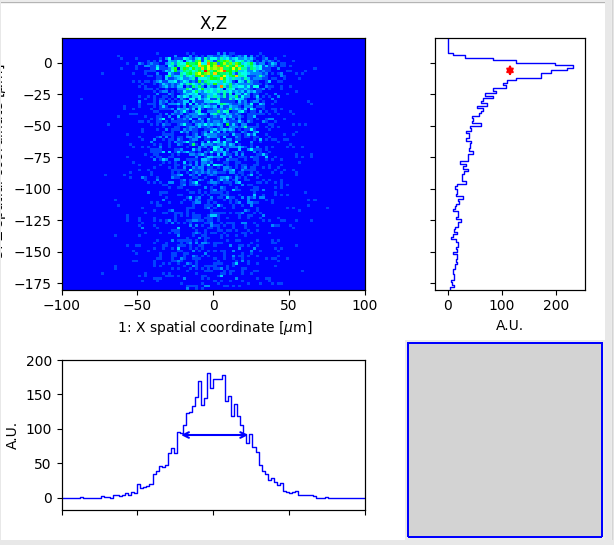
\includegraphics[width=0.49\textwidth]{grazing-mirrors/fig1T.png}
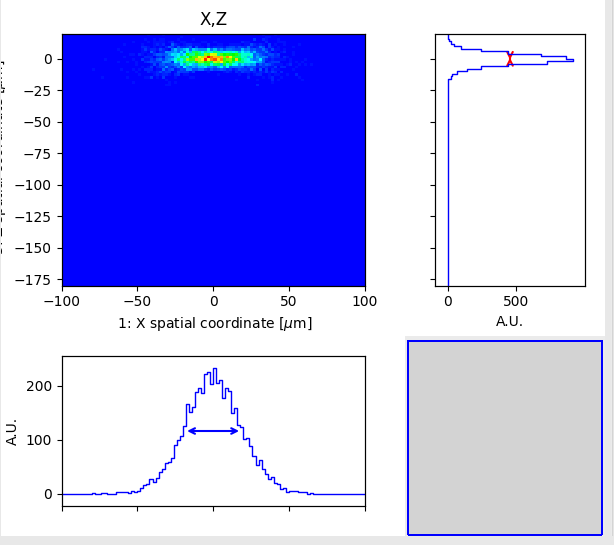
\includegraphics[width=0.49\textwidth]{grazing-mirrors/fig1E.png}
\end{figure}

\begin{figure}[H]
\label{fig:gm-fig2}
\caption{Mirror imaging with magnification M=1/30:  Toroidal (left) and Ellipsoidal (right).}
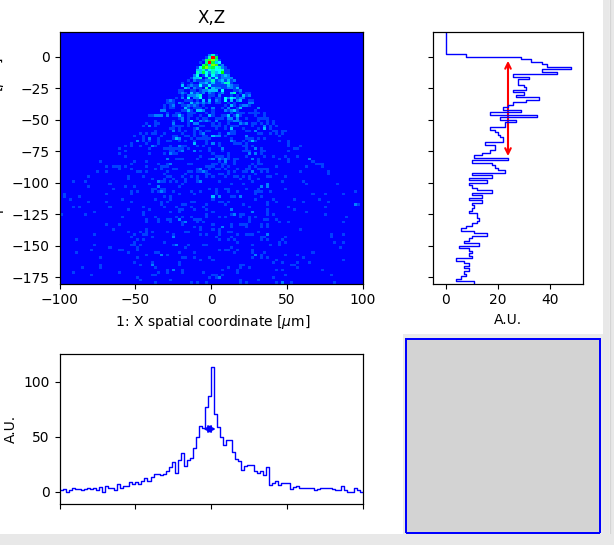
\includegraphics[width=0.49\textwidth]{grazing-mirrors/fig2T.png}
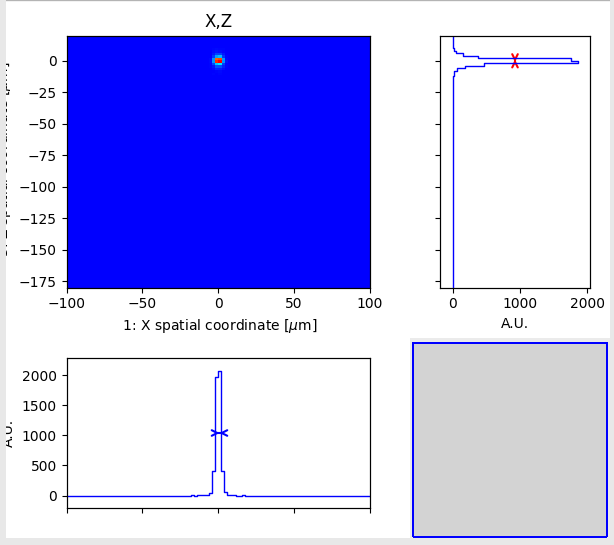
\includegraphics[width=0.49\textwidth]{grazing-mirrors/fig2E.png}
\end{figure}



ii) 

\begin{figure}[H]
\label{fig:gm-fig3}
\caption{I(E) plot from rays (left) or from PreRefl proprocessor (right).}
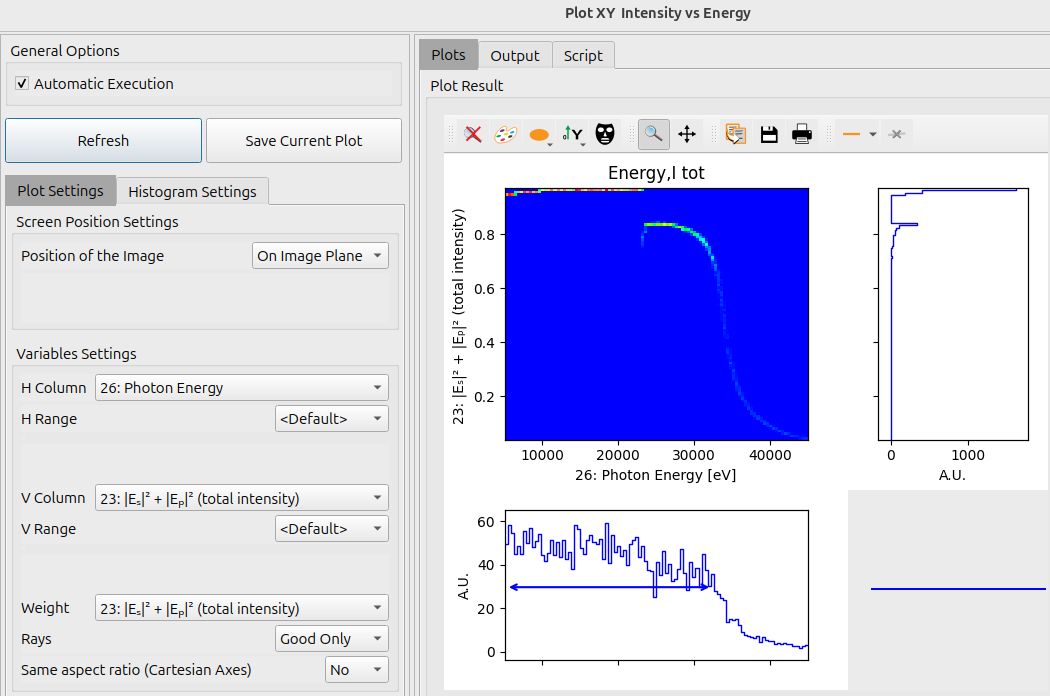
\includegraphics[width=0.49\textwidth]{grazing-mirrors/fig3a.png}
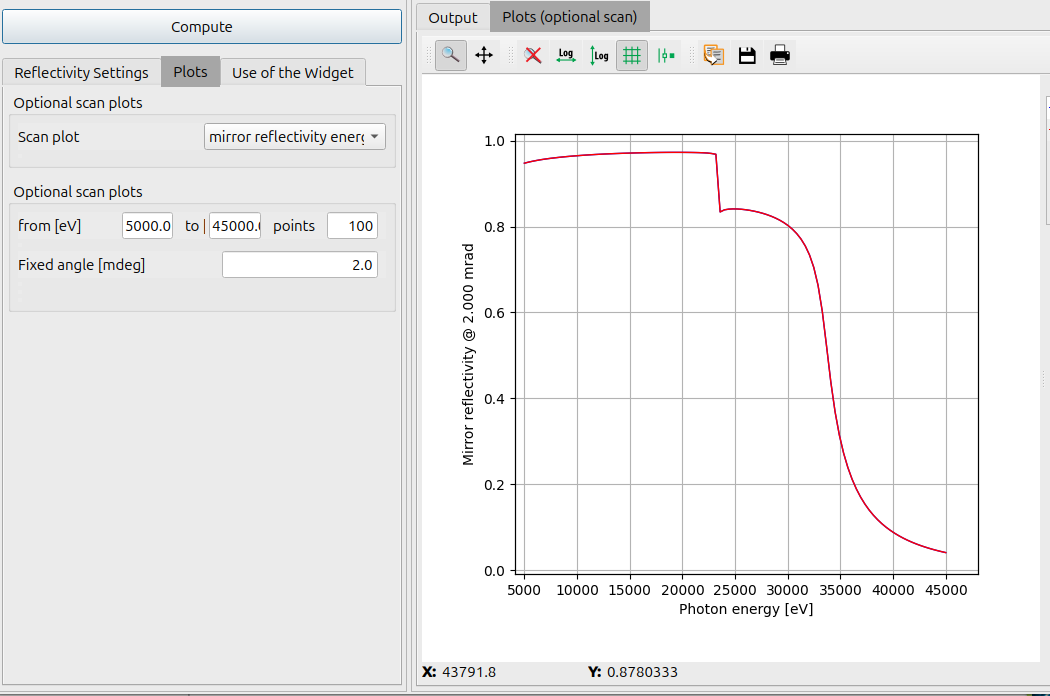
\includegraphics[width=0.49\textwidth]{grazing-mirrors/fig3b.png}
\end{figure}

